%%% Example for master's thesis (in English)
\documentclass[english, dvipdfmx]{ampmt}             % pdflatex
%% \documentclass[dvipdfmx,english]{ampmt} % dvipdfmx

%%% Class options:
%%% chapter:   \chapter command is available (use report.cls).
%%% Options for article or report are also accepted.

%%% Title %%%%%%%%%%%%%%%%%%%%%%%%%%%%%%%%%%%%%%%%%%%%%%%%%%%%%%%%%%%%%%%%%%%%%%%
\title[Deep Reinforcement Learning for Self-Triggered Control]
      {Deep Reinforcement Learning for Self-Triggered Control}
      % [title for spine (option)]{title}
%%% Supervisors %%%%%%%%%%%%%%%%%%%%%%%%%%%%%%%%%%%%%%%%%%%%%%%%%%%%%%%%%%%%%%%%%
\supervisors{Yoshito OHTA}{Professor}             % First supervisor  {name}{title}
            {Kenji KASHIMA}{Assistant Professor} % Second supervisor {name}{title}
            {}{}                               % Third supervisor  {name}{title}
%%% Author %%%%%%%%%%%%%%%%%%%%%%%%%%%%%%%%%%%%%%%%%%%%%%%%%%%%%%%%%%%%%%%%%%%%%%
\author{Ibuki TAKEUCHI}
%%% Submission date %%%%%%%%%%%%%%%%%%%%%%%%%%%%%%%%%%%%%%%%%%%%%%%%%%%%%%%%%%%%%
\submissiondate{2021}{February}   % {year}{month}
%%% Width of a spine %%%%%%%%%%%%%%%%%%%%%%%%%%%%%%%%%%%%%%%%%%%%%%%%%%%%%
\setlength{\wdspine}{15mm}
%%% Number of output spines %%%%%%%%%%%%%%%%%%%%%%%%%%%%%%%%%%%%%%%%%%%%%%%%%%%%%
\def\numberofspines{1}
%%% Abstract %%%%%%%%%%%%%%%%%%%%%%%%%%%%%%%%%%%%%%%%%%%%%%%%%%%%%%%%%%%%%%%%%%%%
\abstract{%
One of the control methods for continuous-time systems is the sample-value control. This is a control method in which the system state is observed and new control inputs are communicated at periodic intervals. The disadvantage of the sample-valued control is that it requires communication at every interval even when the control performance can be maintained without redesigning the control inputs, which results in extra cost for communication.\par
In recent years, event-triggered control and self-triggered control have been focused as control methods for efficient communication and control input design. First of all, event-triggered control is a control method that observes the system state at fixed time intervals as in the case of sample-value control, and redesigns and communicates the control inputs only when the driving conditions are satisfied to achieve the desired control performance. Therefore, it can improve the efficiency in terms of communication cost compared with the sample value control.\par
Next, self-triggered control is described. In the self-triggered control, unlike the sample-value control and the event-triggered control, the periodic state observation is not performed. Instead, the designer itself decides the next trigger time and communicates the state observation and control input after that time. For the self-triggered control, several model-based design methods have been proposed, but these methods do not explicitly consider the communication cost over a long time of control.\par
In this paper, we formulate an optimal self-triggered control problem where communication cost is explicitly included, which has not been considered in previous studies. Then, we consider a policy gradient method to the problem formulated in this paper.\par
We also propose a reinforcement learning algorithm for approximate computation of the policy gradient. As a result of the implementation, for the linear system, we can improve the policy from the control law designed naively in the model based method. We also succeeded in improving the policy from periodic control for self-triggered control of nonlinear systems, which was not solved in the previous study.\par
}
%%% Packages and definitions of your own macros %%%%%%%%%%%%%%%%%%%%%%%%%%%%%%%%%
\newcommand{\rme}{\mathrm{e}}
%\usepackage[top=20truemm,bottom=20truemm,left=25truemm,right=25truemm]{geometry}
\usepackage{amsmath,ascmac,url,amsfonts,bm,here,algorithmic,algorithm,amsthm,color}
\newcommand{\unc}[1]{\textcolor{red}{#1}} %unconfirmed data
\newcommand{\argmax}{\mathop{\rm argmax}\limits}
\newcommand{\argmin}{\mathop{\rm argmin}\limits} 
\newcommand{\expect}{\mathbb{E}} 
\newcommand{\trans}[1]{#1^{\top}}
\newcommand{\pdif}[2]{\frac{\partial#1}{\partial#2}}
\newcommand{\odif}[2]{\frac{\rm{d}#1}{\rm{d}#2}}
\newtheorem{th.}{Theorem}
\renewcommand\proofname{\bf Proof}


%%% Control of output %%%%%%%%%%%%%%%%%%%%%%%%%%%%%%%%%%%%%%%%%%%%%%%%%%%%%%%%%%%

%%% If you don't want to output body text, activate the next line.
%% \outputbodyfalse

%%% If you don't want to output covers at the end of PDF, activate the next line.
%% \outputcoverfalse

%%% If you don't want to output abstract for submission at the end of PDF,
%%% activate the next line.
%% \outputabstractforsubmissionfalse

%%% If you want to change the layout, use \geometry command provided by
%%% the geometry package.
%% \geometry{hmargin=3cm,vmargin=2cm}

\begin{document}
\ifoutputbody
%%% Inside cover, abstract and table of contents %%%%%%%%%%%%%%%%%%%%%%%%%%%%%%%%
\makeinsidecover                % Inside cover
\makeabstract                   % Abstract
\maketoc                        % Table of contents
\setcounter{page}{1}
%%% Body %%%%%%%%%%%%%%%%%%%%%%%%%%%%%%%%%%%%%%%%%%%%%%%%%%%%%%%%%%%%%%%%%%%%%%%%
\section{Introduction}
One of the control methods for continuous-time systems is the sample-value control. This is a control method in which the system state is observed and new control inputs are communicated at periodic intervals. The disadvantage of the sample-valued control is that it requires communication at every interval even when the control performance can be maintained without redesigning the control inputs, which results in extra cost for communication.\par
In recent years, event-triggered control and self-triggered control have been focused as control methods for efficient communication and control input design. First of all, event-triggered control is a control method that observes the system state at fixed time intervals as in the case of sample-value control, and redesigns and communicates the control inputs only when the driving conditions are satisfied to achieve the desired control performance. Therefore, it can improve the efficiency in terms of communication cost compared with the sample value control. For event-triggered control, several model-based design methods introduced in \cite{ETC_intro} have been proposed, and model-free methods using reinforcement learning such as \cite{ETC} have also been proposed.\par
Next, self-triggered control is described. In the self-triggered control, unlike the sample-value control and the event-triggered control, the periodic state observation is not performed. Instead, the designer itself decides the next trigger time and communicates the state observation and control input after that time. For the self-triggered control, model-based design methods have been proposed in \cite{STC} and \cite{ECBF}. However, these methods do not explicitly consider the communication cost over a long time of control.\par
By the way, artificial intelligence is nowadays used in various situations, notably in automatic driving technology, and the development of research on the subject of artificial intelligence is remarkable. One of the concepts to realize artificial intelligence is reinforcement learning. Reinforcement learning is an algorithm that learns behaviors that optimize the long-term benefits by repeated trial and error. In addition, although not mathematically proven, reinforcement learning has been used to obtain meaningful results for nonlinear systems. In this paper, we investigate the usefulness of reinforcement learning as a method to realize the self-triggered control law. \par
The two main contributions of this research are
\begin{itemize}
	\item To formulate the optimal self-triggered control problem for long-time costs explicitly considering communication cost, and to consider the policy gradient for it.
	\item To confirm the usefulness of reinforcement learning for self-triggered control not only for linear systems but also for non-linear systems.
\end{itemize}

\section{Preliminaries}
\subsection{Background of Deep Reinforcement Learning}
Consider a malkov decision process $M$ given with tuple $M=\{S,A,TP,d_0,r,\gamma\}$. Here, $S,A$ denotes state, action set, and $TP(s^{'}|s,a)$ express transition probability. Also, $d_0,r(s,a),\gamma\in[0,1]$ are distribution of initial state, reward, discount factor respectively. \par
The purpose of reinforcement learning is to find a policy such that
\begin{equation}
	\pi^{*}=\argmax_{\pi}J(\pi) \label{purpose_of_rl}
\end{equation} 
where evaluation function $J(\pi)$ and (state) value function $V^{\pi}(s)$ is given as following:
\begin{align}
	V^{\pi}(s) &= \expect_{TP}\left[\sum_{t=0}^{\infty}\gamma^tr(s_t, a_t)|_{a_t=\pi(s_t)}, s_0 = s\right]\\
	J(\pi) &= \expect_{s_0\sim d_0}[V^{\pi}(s_0)]
\end{align}
The expectation $\expect_{TP}$ takes over the transition probability.\par
Let us define $Q$ function, which is useful tool for analyzing reinforcement learning. $Q$ function is given as 
\begin{align}
	Q^{\pi}(s,a) &= r(s, a) + \gamma\expect_{TP}\left[\sum_{t=1}^{\infty}\gamma^tr(s_t, a_t)|_{a_t=\pi(s_t)} \right]\nonumber\\
			    &= r(s, a) + \gamma \expect_{TP}[V^{\pi}(s^{\prime})]. \label{Q_func}
\end{align}
As shown in \eqref{Q_func}, $Q$ function express the value when the agent select action $a$ freely and choose action according to the policy $\pi$ from the next step. Thus, the $Q$-function is also known as the action value function.


\subsection{Policy Iteration}
There is an algorithm for achieving \eqref{purpose_of_rl}, called the policy iteration method. It consists of repeating the following two steps.
\begin{enumerate}
	\item Policy Evaluation: Find (or approximate) action value function $Q^{\pi}(s,a)$.
	\item Policy Improvement: Update policy as $\pi(s)=\argmax_aQ^{\pi}(s,a)$.
\end{enumerate}
It is known that the optimal policy $\pi^{*}$ can be obtained by repeating the above two steps (Policy Improvement Theorem).%文献

\subsection{Algorithms adapted to the settings of state and action space}
\label{sec:policy_improvement}
In the case that both the state space and the action space take discrete values, it is easy to obtain
$\pi(s)=\argmax_aQ^{\pi}(s,a)$ by storing $Q^{\pi}(s,a)$ in a table.\par
Now, what about the case where the state space is continuous? Since the state $s$ takes a continuous value, it cannot be stored in a table. Therefore, Minh et al.\cite{DQN} took the approach of approximating $Q^{\pi}(s,a)$ by parametrizing it using a neural network. Since the action space is discrete, it is still possible to obtain $\argmax_aQ^{\pi}(s,a)$. \par
Finally, in the case where both state and action space is continuous, the problem is that it is very expensive to obtain $\argmax_aQ^{\pi}(s,a)$. Thus, up to this point, the policy $\pi$ has been determined by the Q-function, but this approach cannot be taken when both spaces are continuous. 
Therefore, the policy function is often parameterized as $\pi_{\theta}$ and the parameter $\theta$ is updated by gradient mothod. 

\subsection{Deterministic Policy Gradient Method}
Silver et al.\cite{DPG} finds the gradient for the evaluation function $J(\pi_{\theta})$, even if the policy $\pi(s)$ is defined as deterministic policy. This gradient is known as deteministic policy gradient(DPG), and it is calculate as following theorem.
\begin{th.}[Deterministic Policy Gradient Theorem]
The gradient for evaluation function $\nabla_{\theta}J(\pi_{\theta})$ is exist and calculated as, 
\begin{align}
	\nabla_{\theta}J(\pi_{\theta}) &= \expect_{s\sim\rho^{\pi_{\theta}}}[
	\nabla_{\theta}\pi_{\theta}(s)\nabla_{a}Q^{\pi_{\theta}}(s, a)|_{a=\pi_{\theta}(s)}] \label{true_pg} 
\end{align}
where, 
\begin{equation}
	\rho^{\pi_{\theta}}(s) = \int_{S}\sum_{t=0}^{\infty}\gamma^td_0(s_0)\textrm{Pr}(s_0\to s, t,  \pi_{\theta})\textrm{d}s_0
\end{equation}
is discounted distribution.
\end{th.}
\begin{proof}
First, we consider the gradient for $V^{\pi_{\theta}}(s)$.
\begin{align}
	& \nabla_{\theta}V^{\pi_{\theta}}(s) \nonumber \\ 
	&= \nabla_{\theta}Q^{\pi_{\theta}}(s, \pi_{\theta}(s))\nonumber\\
	&= \nabla_{\theta}[r(s,\pi_{\theta}(s))+\gamma\int_{S}Pr(s\to s^{\prime}, 1, \pi_{\theta})V^{\pi_{\theta}}(s^{\prime})ds^{\prime}] \nonumber\\
	&= \nabla_{\theta}\pi_{\theta}(s)\nabla_{a}r(s,a)|_{a=\pi_{\theta}(s)} \nonumber \\
	&\hspace{1ex}+\gamma\int_{S}(\nabla_{\theta}\pi_{\theta}(s)\nabla_aPr(s\to s^{\prime},1,a)|_{a=\pi(s)}V^{\pi_{\theta}(s^{\prime})}\nonumber\\
	&\hspace{1ex}+Pr(s\to s^{\prime}, 1, \pi_{\theta})\nabla_{\theta}V^{\pi_{\theta}}(s^{\prime}))ds^{\prime}\nonumber\\
	&= \nabla_{\theta}\pi_{\theta}(s)\nabla_a[r(s,a)+\gamma\int_{S}Pr(s\to s^{\prime}, 1, \pi_{\theta})V^{\pi_{\theta}}(s^{\prime})]_{a=\pi_{\theta(s)}}ds^{\prime} \nonumber \\
	&\hspace{1ex}+\gamma\int_{S}Pr(s\to s^{\prime}, 1, \pi_{\theta})\nabla_{\theta}V^{\pi_{\theta}}(s^{\prime})ds^{\prime}\nonumber\\
	&= \nabla_{\theta}\pi_{\theta}(s)\nabla_aQ^{\pi_{\theta}}(s,a)|_{a=\pi_{\theta}(s)} + \gamma\int_{S}Pr(s\to s^{\prime}, 1, \pi_{\theta})\nabla_{\theta}V^{\pi_{\theta}}(s^{\prime})ds^{\prime}
\end{align}
By using this relation recursively, we have,
\begin{align}
	\nabla_{\theta}V^{\pi_{\theta}}(s) &= \sum_{i=0}^{\infty}\int_{S}\cdots\int_{S}Pr(s\to s^{\prime},1,\pi_{\theta})Pr(s^{\prime}\to s^{\prime\prime},1,\pi_{\theta})\cdots\nonumber\\
	&\hspace{10ex}\gamma^i\nabla_{\theta}\pi_{\theta}(s^{\prime\cdots\prime})\nabla_aQ^{\pi_{\theta}}(s^{\prime\cdots\prime},a)|_{a=\pi_{\theta}(s^{\prime\cdots\prime})}ds^{\prime\cdots\prime}\ldots ds^{\prime}\nonumber\\
	&= \sum_{i=0}^{\infty} \gamma^i\int_{S}Pr(s\to s^{\prime}, i, \pi_{\theta})\nabla_{\theta}\pi_{\theta}(s)\nabla_aQ^{\pi_{\theta}}(s,a)|_{a=\pi_{\theta}(s^{\prime})}ds^{\prime}.\label{multiple_integral}
\end{align}
Since $J(\pi) = \expect_{s\sim d_0}[V^{\pi}(s)]$, 
\begin{align}
	\nabla_{\theta}J(\pi_{\theta}) &= \nabla_{\theta}\int_{S}d_0(s)V^{\pi_{\theta}}(s)ds \nonumber\\
	&= \int_{S}d_0(s)\nabla_{\theta}V^{\pi_{\theta}}(s)ds \nonumber\\
	&= \int_{S}\rho^{\pi_{\theta}}\nabla_{\theta}\pi_{\theta}(s)\nabla_aQ^{\pi_{\theta}}(s,a)|_{a=\pi_{\theta}(s)}ds
\end{align}
\end{proof}

DDPG(Deep DPG) is a deep reinforcement learning algorithm which utilize this policy gradient. It adopts an Actor-Critic structure, and learns a critic network $Q(s,a|\omega)$ which approximates $Q^{\pi_{\theta}}$, and an actor network $\pi(s|\theta)=\pi_{\theta}$ which represents a policy $\pi$, respectively. The update algorithm of actor and critic is described below.\par
DDPG uses mini-batch learning. First, update idea of critic is shown. The purpose of critic is to approximate $Q^{\pi}$. Because $Q$ function is able to be decomposed like \eqref{Q_func}, $Q(s,a|\omega)$ should also be updated to satisfy this relation. For that, parameter $\omega$ is updated to the direction where it minimize Temporal Difference(TD) error: 
\begin{equation}
	Q(s,a|\omega) - \{r(s,a)+\gamma \expect_{s^{\prime}}[Q(s^{\prime},\pi(s^{\prime})|\omega)]\}
\end{equation}
Since it is difficult to optimize for whole $(s,a)$ at once, DDPG uses the mean squared error for the mini-batch $E$ as the loss function and reduces it. 
\begin{equation}
	Loss = \frac{1}{N}\sum_{(s,a,s^{\prime})\in E} \{Q(s,a|\omega) - (r(s,a)+\gamma Q(s^{\prime},\pi(s^{\prime})|\omega))\}^2
\end{equation}\par
Now, the above method of updating critic is supervised learning itself. Therefore, the data in the mini-batch must be i.i.d.. If the mini-batch $E$ uses the data of the last $N$ steps experienced by the agent, they are no longer independent. Hence, the agent stores the empirical data in a storage, called replay buffer, and randomly selects $N$ data from it to make a mini-batch to increase the variance of it.\par
Next update law of actor are shown. Because actor is the representation of policy function $\pi(s)$, policy gradient is used for its update. However, since correct $Q$-function as in equation \eqref{true_pg} cannot be used in DDPG, approximated policy gradient
\begin{equation}
	\expect_{s\sim\rho^{\pi}}[\nabla_{\theta}\pi_{\theta}(s)\nabla_{a}Q(s, a|\omega)|_{a=\pi_{\theta}(s)}] \simeq \nabla_{\theta}J(\pi_{\theta}) 
\end{equation}
 is used. Furthurmore, an approximation to the expectation is made like following:
 \begin{equation}
	\expect_{s\sim\rho^{\pi}}[\nabla_{\theta}\pi_{\theta}(s)\nabla_{a}Q(s, a|\omega)|_{a=\pi_{\theta}(s)}] \simeq \frac{1}{N}\sum_{s\in E}[\nabla_{\theta}\pi_{\theta}(s)\nabla_{a}Q(s, a|\omega)|_{a=\pi_{\theta}(s)}]. \label{expectation_approximation}
\end{equation}
Therefore, the accuracy of the approximation of the policy gradient may be greatly degraded by the accuracy of critic approximation and the distribution of mini-batch.


\section{Problem Formulation}
\subsection{Self-Triggered Control}
We consider control system like Fig \ref{image}.
\begin{figure}[h]
	\centering
 	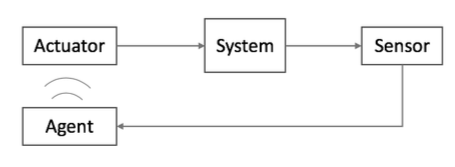
\includegraphics[width=10cm]{event.png}
 	\caption{control system} \label{image}
\end{figure}\\
Here, the control target is a continuous-time system as Equation \eqref{continuous_system}
\begin{equation}
	\dot{s} = h(s,u) + \dot{w}\label{continuous_system}.
\end{equation}\par
Now, we consider a feedback control for system \eqref{continuous_system}. In this paper, we call the observation of the state variable $s$ and the sending of the input signal to the actuator as "interaction". In the self-triggered control, the agent does not make interaction continuously, but after a communication interval $\tau$ seconds determined by the agent itself. In order to express it mathematically, we assume that the agent's control law $\pi$ is a vector-valued function consisting of two elements, where the first element represents the input $u$ sent to the actuator, and the second element represents the interval $\tau$ seconds. The input $u$ sent in the previous interaction is added until the time of the next interaction (Zero Order Hold control).

\subsection{Previous Research for Self-Triggered Control}
Previous researches in self-triggered control utilizing a Lyapunov function approach, such as \cite{STC} and \cite{ECBF}, make one step optimization of the next triggering time on each interaction.  However, this approach does not satisfy the optimality for the whole long time control episode. \par
In this research, we formulate an optimal self-triggered control problem in which communication is explicitly included in the cost. This makes it possible to consider the problem of finding a control policy with a long-term cost, instead of a one-step optimization.

\subsection{Optimal Self-Triggered Control}
\label{sec:formulation}
In self-triggered control, the agent needs to decide the input signal $u$ and the interval $\tau$ at each step. Thus, the action $a$ in reinforcement learning corresponds to $\begin{bmatrix}u & \tau \end{bmatrix}^{\top}$. (In this paper, we equate $a$ with the tuple $(u,\tau)$.) \par
Now, in this research, the control law is given as a state feedback. Therefore, the policy function is given as follows:
\begin{equation}
	\pi(s) = \begin{bmatrix}u(s) & \tau(s)\end{bmatrix}^{\top}
\end{equation}\par
In order to converge to the origin state as quickly as possible with the minimum input energy while reducing the frequency of communication, the agent aims to find a policy $\pi^{*}$ that minimizes the following expected discounted cost 
\begin{equation}
	J(\pi)=\expect_{s\sim d_0}[V^{\pi}(s)] \label{evaluation}
\end{equation}
where
\begin{equation}
	V^{\pi}(s) = \int_{0}^{\infty} e^{-\alpha t}\expect_{w}[s(t)^{\top}Qs(t)+u(t)^{\top}Ru(t)+\beta C(t)|s(0)=s]\textrm{d}t \label{such_that}
\end{equation}
and $C(t)$ is a boolean function which denotes the agent interact at time $t$.\par
If we separate the definite integral for each interval, we have 
\begin{align}
	V^{\pi}(s) &= \sum_{i=0}^{\infty}\int_{t_i}^{t_{i+1}} e^{-\alpha t}\expect_{w}[s(t)^{\top}Qs(t)+u_i^{\top}Ru_i+\beta C(t)|s(0)=s]\textrm{d}t \nonumber \\
			 &= \sum_{i=0}^{\infty} e^{-\alpha t_i} \left(\int_{0}^{\tau_i}e^{-\alpha t}\expect_{w}[s(t)^{\top}Qs(t)+u_i^{\top}Ru_i|s(0)=s_i]\textrm{d}t + \beta\right) \nonumber \\
			 &= \sum_{i=0}^{\infty} e^{-\alpha t_i} r(s_i, \pi(s_i)) \label{self_acc_reward}.
\end{align}
Here, $t_i$ is the time of the $i$-th communication and $s_i$ is the state at that time. Also, let $[u_i, \tau_i]=\pi(s_i)$, and let be the reward function $r(s_i, u_i, \tau_i)$ of each steps as
\begin{equation}
	r(s_i, u_i, \tau_i) = \int_{0}^{\tau_i}e^{-\alpha t}\expect_{w}[s(t)^{\top}Qs(t)+u_i^{\top}Ru_i|s(0)=s_i]\textrm{d}t + \beta
\end{equation}

Therefore, $V^{\pi}(s)$ satisfies the following Bellman equation. \par
\begin{equation}
	V^{\pi}(s) = r(s,\pi_{\theta}(s)) + e^{-\alpha\tau}\expect_{s^{\prime}}[V^{\pi}(s^{\prime}(s,\pi_{\theta}(s)))] \label{bellman}
\end{equation}
In addition, the action value function $Q^{\pi}$ is the discounted accumulation cost when agent freely chooses an action in the first step and follows the policy $\pi$ from the next step, which satisfies the following Bellman equation.
\begin{equation}
	Q^{\pi}(s,u,\tau) = r(s,u,\tau) + e^{-\alpha\tau}\expect_{s^{\prime}}[Q^{\pi}(s^{\prime}(s,u,\tau), \pi(s^{\prime}(s,u,\tau)))] \label{Q_bellman}
\end{equation}


\section{Reinforcement Learning for Self-Triggered Control}
In this section, we consider the application of reinforcement learning to find the optimal self-trigger policy $\pi^{*}$. Simply thinking, we can consider the reinforcement learning problem by taking the interaction as one step. Furthermore, DDPG may also be applied by approximating the $Q$-function, which satisfies the equation \eqref{Q_bellman} using a critic network, to obtain the policy gradient. In this section, we discuss the validity of this approach.

\subsection{Deterministic Policy Gradient for Self-Triggered Control}
Since the discount factor in Equation \eqref{self_acc_reward} depends on $\tau$ at each step, it differs from the general reinforcement learning problem. In this subsection, we discuss how the DPG is affected by this difference. \par
Actually, due to the property of $Q$-functions such as \eqref{Q_bellman}, DPG cannot be computed as in \eqref{true_pg}. Since 
\begin{align}
	\nabla_{\theta}V^{\pi_{\theta}}(s) &= \nabla_{\theta}Q^{\pi_{\theta}}(s, \pi_{\theta}(s)) \nonumber \\
	&= \nabla_{\theta}[r(s, \pi_{\theta}(s)) + e^{-\alpha\tau_{\theta}(s)}\expect_{s^{\prime}}[V^{\pi_{\theta}}(s^{\prime})] \nonumber \\
	&= \nabla_{\theta}\pi_{\theta}(s)\nabla_ar(s,a)|_{a=\pi_{\theta}(s)} \nonumber \\
	&\hspace{1ex}+e^{-\alpha\tau_{\theta}(s)}\int_{S}\{\nabla_{\theta}\pi_{\theta}(s)\nabla_aPr(s\to s^{\prime},1,a)|_{a=\pi(s)}V^{\pi_{\theta}}(s^{\prime})\nonumber\\
	&\hspace{15ex}+Pr(s\to s^{\prime}, 1, \pi_{\theta})\nabla_{\theta}V^{\pi_{\theta}}(s^{\prime})\}ds^{\prime}\nonumber \\
	&\hspace{1ex}+\int_{S}\nabla_{\theta}e^{-\alpha\tau_{\theta}(s)}Pr(s\to s^{\prime}, 1, \pi_{\theta})V^{\pi_{\theta}}(s^{\prime})ds^{\prime},
\end{align}
we have
\begin{align}
	&\nabla_{\theta}V^{\pi_{\theta}}(s) \nonumber \\
	&= \sum_{i=0}^{\infty}\int_{S}\cdots\int_{S}Pr(s_0\to s_1,1,\pi_{\theta})\cdots Pr(s_{i-1}\to s_i,1,\pi_{\theta})\nonumber\\
	&\hspace{10ex}e^{-\alpha t_i}\nabla_{\theta}\pi_{\theta}(s_i)\nabla_aQ^{\pi_{\theta}}(s,a)|_{a=\pi_{\theta}(s_i)}ds_ids_{i-1}\ldots ds_1\nonumber\\
	&\hspace{1ex}+\sum_{i=1}^{\infty}\int_{S}\cdots\int_{S}Pr(s_0\to s_1,1,\pi_{\theta})\cdots Pr(s_{i-1}\to s_i,1,\pi_{\theta})\nonumber\\
	&\hspace{10ex}e^{-\alpha t_{i-1}}\nabla_{\theta}e^{-\alpha\tau_{\theta}(s_{i-1})}V^{\pi_{\theta}}(s_{i})ds_ids_{i-1}\ldots ds_1\nonumber\\
	&= \sum_{i=0}^{\infty}\int_{S}\cdots\int_{S}Pr(s_0\to s_1,1,\pi_{\theta})\cdots Pr(s_{i-1}\to s_i,1,\pi_{\theta})\nonumber\\
	&\hspace{10ex}e^{-\alpha t_i}\nabla_{\theta}\pi_{\theta}(s_i)\nabla_aQ^{\pi_{\theta}}(s,a)|_{a=\pi_{\theta}(s_i)}ds_ids_{i-1}\ldots ds_1\nonumber\\
	&\hspace{1ex}+\sum_{i=0}^{\infty}\int_{S}\cdots\int_{S}Pr(s_0\to s_1,1,\pi_{\theta})\cdots Pr(s_{i}\to s_{i+1},1,\pi_{\theta})\nonumber\\
	&\hspace{10ex}e^{-\alpha t_{i}}\nabla_{\theta}e^{-\alpha\tau_{\theta}(s_{i})}V^{\pi_{\theta}}(s_{i+1})ds_{i+1}ds_{i}\ldots ds_1,
\end{align}
where 
\begin{equation}
	t_i = \begin{cases}
    		0 & (i=0) \\
    		\sum_{k=0}^{i-1}\tau_{\theta}(s_{k-1}) & (otherwise)
  		\end{cases}.
\end{equation}\par
Now, since $J(\pi_{\theta}) = \expect_{s_0\sim d_0}[V^{\pi_{\theta}}(s_0)]$, we have deterministic policy gradient theorem for self-triggered control.

\begin{th.}[Deterministic Policy Gradient Theorem for Self-Triggered Control]
The gradient for evaluation function \eqref{evaluation}, \eqref{such_that} is calculated as, 
\begin{align}
	&\nabla_{\theta}J(\pi_{\theta})\nonumber \\
	&= \expect_{s_0\sim d_0}[\nabla_{\theta}V^{\pi_{\theta}}(s_0)]\nonumber\\
	&= \sum_{i=0}^{\infty}\int_{S}\cdots\int_{S}d_0(s_0)Pr(s_0\to s_1,1,\pi_{\theta})\cdots Pr(s_{i}\to s_{i+1},1,\pi_{\theta})\nonumber\\
	&\hspace{5ex}e^{-\alpha t_i}\{\nabla_{\theta}\pi_{\theta}(s_i)\nabla_aQ^{\pi_{\theta}}(s,a)|_{a=\pi_{\theta}(s_i)} + \nabla_{\theta}e^{-\alpha\tau_{\theta}(s_{i})}V^{\pi_{\theta}}(s_{i+1})\}ds_{i+1}ds_{i}\ldots ds_0. \label{PG_for_STC}
\end{align}
\end{th.}

\subsection{Value function for Self-Triggered Control}
In DPG for reinforcement learning problems with a fixed discount factor, it is sufficient that the gradient of the critic $Q(s,a|\omega)$ with respect to $a$ can correctly approximate that of the $Q$-function. However, in the case of reinforcement learning for self-triggered control considered in this paper, the value of $Q(s,\pi(s)|\omega)$ itself must also be correctly approximated. Therefore, we need to pay attention to the TD learning of critic.\par
In this section, we discuss whether the critic learned using TD learning can approximate the value of $Q^{\pi}(s,a)$. First of all, since the Bellman equation for the $Q$-function in self-triggered control should satisfy \eqref{Q_bellman}, the critic should set the TD error
\begin{equation}
	TD = Q(s,u,\tau|\omega) - \{r(s,u,\tau) + e^{-\alpha\tau}\expect_{s^{\prime}}[Q(s^{\prime}(s,u,\tau), \pi(s^{\prime}(s,u,\tau))|\omega)]\}
\end{equation}
 to be zero for all $(s,u,\tau)$. In this section, we discuss the algorithm for learning such a critic.\par
Here, we create a mini-batch $E$ from the dataset $D={(s,u,\tau,r,s)}$ and learn critic by minimizing the MSE of the TD error for the mini-batch $E$. Therefore, if there is a bias of the distribution of $(s,u,\tau)$ in the empirical data set $D$, the accuracy of function approximation outside the distribution will obviously be low. From the equation \eqref{PG_for_STC}, the approximation of $Q(s, \pi(s)|\omega)$ and $\nabla_aQ(s,a|\omega)|_{a=\pi(s)}$ is necessary for the calculation of the directional gradient, so we create a dataset $D$ which contains $s$ in the whole region of $S$ and $[u,\tau] = \pi(s) + e $ (where $e$ is a stochastic noise)\par
Algorithm \ref{alg1} shows the learning algorithm for critics described in this section.
\begin{algorithm}                      
\caption{TD Learning for Critic Network}         
\label{alg1}                          
\begin{algorithmic}                  
    \STATE Sample $M$ states $s$ with equal probability from state space $S$.
    \FOR {$r = 0$ to $R$}
    	\STATE For all sampled $s$, choose $[u, \tau]=\pi(s) + e$.
	\STATE Execute action $u$ for $\tau$ second to the environment.
	\STATE Receive $r$ and observe next state $s^{\prime}$.
	\STATE Store $(s, u, \tau, r, s^{\prime})$ to data set D.
    \ENDFOR
    \FOR {$\textrm{epoch} = 0$ to $N$}
    	\STATE Select $m$ data pairs $(s, u, \tau, r, s^{\prime})$ from $D$ and make a mini-batch $E$.
	\STATE Calculate gradient $g = \pdif{}{\omega} \frac{1}{m}\sum_{E}\left(Q(s,u,\tau|\omega) - \{r + e^{-\alpha\tau}Q(s^{\prime}, \pi(s^{\prime})|\omega)\}\right)^2$.
	\STATE Update $\omega$ with gradient $g$.
    \ENDFOR
    \end{algorithmic}
\end{algorithm}\\
In the last part of this section, we compare $Q^{\pi}(s, \pi(s))$ for a self-triggered control law $\pi$ with the critic $Q(s,\pi(s)|\omega)$ which approximates $Q^{\pi}(s, \pi(s))$ using the algorithm \ref{alg1}. Both $Q^{\pi}(s, \pi(s))$ and $Q(s, \pi(s)|\omega)$ are functions of state $s$. The state $s$ is assumed to be two-dimensional, and the comparison between them is shown in Figure \ref{Q_approximation}. 
\begin{figure}[H]
	\centering
 	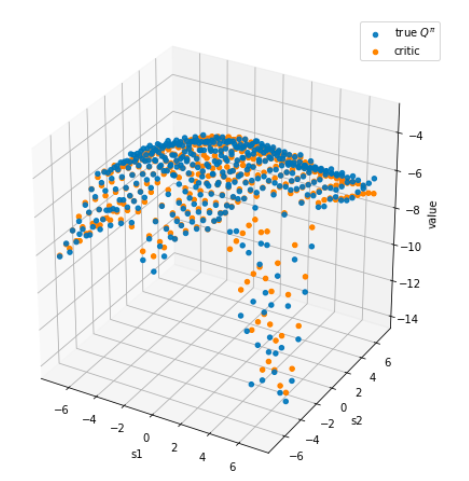
\includegraphics[width=10cm]{Q_approximation.png}
 	\caption{Approximation of $Q^{\pi}(s,\pi(s))$} \label{Q_approximation}
\end{figure}
In Figure \ref{Q_approximation}, the blue points indicate the true $Q^{\pi}$ and the orange points indicate the critics. The true $Q^{\pi}$ is obtained by simulation. From Figure \ref{Q_approximation}, we can see that the critic learned by Algorithm \ref{alg1} is a good approximation of $Q^{\pi}$.


\subsection{Ideal Algorithm}
We start by considering an ideal algorithm for computing the exact policy gradient \eqref{PG_for_STC} without considering the computational complexity. First, for an initial state $s_0$, we perform $P$ episodes of control for $T$ seconds.  In each step, we store $(s_i, u_i, \tau_i, r_i, t_i)$ in a set. The difference with DDPG is that the time at each step is also stored. When let $T_i$ be the set $\{i~|~t_i \leq T\}$. for each control path, we can approximate $\nabla_{\theta}V^{\pi_{\theta}}(s_0)$ by computing 
\begin{equation}
	\sum_{i\in T_i} e^{-\alpha t_i}\{\nabla_{\theta}\pi_{\theta}(s_i)\nabla_{a}Q(s,a|\omega)|_{a=\pi_{\theta}(s_i)} + \nabla_{\theta}e^{-\alpha\tau_{\theta}(s_{i})}Q(s_{i+1},\pi_{\theta}(s_{i+1})|\omega)\} \label{good_approximation_of_STCDPG}
\end{equation}
and averaging it over $P$ paths. We can approximate the policy gradient by generating $M$ initial states $s_0$ from the initial state distribution $d_0$ and taking the average of this calculation for each of them. If we take $P, N$ and $M$ to be infinitely large, and if $Q(s,a|\omega)$ is a good approximation of $Q^{\pi_{\theta}}(s,a)$, we can calculate the correct policy gradient.\par
In algorighm \ref{alg2}, the reinforcement learning method with ideal calculation of policy gradient at each step. 
\begin{algorithm}                      
\caption{Ideal Algorithm for Self-Triggered Control RL}         
\label{alg2}                          
\begin{algorithmic}                  
    \STATE Initialize actor $\pi_{\theta}(s)$ and critic $Q(s,u,\tau|\omega)$.
    \STATE Make target networks $\pi_{\theta^{\prime}}(s)$ and critic $Q(s,u,\tau|\omega^{\prime})$ by cloning actor and critic respectively.
    \STATE Learn critic $Q(s,u,\tau|\omega)$ with algorithm \ref{alg1}.
    \FOR {$epoch=0$ to $N$}
        \FOR {$m = 0$ to $M$}
            \STATE Initialize $s_0\sim d_0$.
        \FOR {$\textrm{episode} = 0$ to $P$}
            \STATE Initialize episode memory $E$.
                \WHILE {$t \leq T$}
                \STATE Select $[u, \tau] = \pi_{\theta}(s)$.
                \STATE Execute action $u$ for $\tau$ second to the environment.
                \STATE Receive $r$ and observe next state $s^{\prime}$.
                \STATE Store tuple $(s, u, \tau, r, s^{\prime}, t)$.
            \ENDWHILE
            \STATE Calculate \eqref{good_approximation_of_STCDPG} with episode memory $E$.
        \ENDFOR
        \STATE Take the average of \eqref{good_approximation_of_STCDPG} over P paths, and let it be $V^{\pi_{\theta}}(s_0)$.
        \ENDFOR
    \ENDFOR
    \STATE Take the average of $V^{\pi_{\theta}}(s_0)$ over the generated $s_0$ and let it be policy gradient $g$.
    \STATE Update actor with approximated policy gradient $g$.
   \STATE Update target network.
   \end{algorithmic}
\end{algorithm}

\subsection{Practical Algorighm}
As I mentioned before, the above algorithm does not take into account the problem of computational complexity. Therefore, from now on, we consider an efficient method to approximate the policy gradient. The most important point is the state distribution of the mini-batch which takes the sample mean to approximate equation \eqref{PG_for_STC}. \par
Assuming that the update of the actor is very gradual, the replay buffer stores the experience gained by policies similar to the current policy. Thus, for each experience $(s_i, u_i, \tau_i, r_i, t_i)$, if we create a mini-batch $E$ by sampling the experience with probability $e^{-\alpha t_i}$, we can expect that the sample mean
\begin{equation}
	\frac{1}{N}\sum_{(s, s^{\prime})\in E}\{\nabla_{\theta}\pi_{\theta}(s)\nabla_{a}Q(s,a|\omega)|_{a=\pi_{\theta}(s)}+\nabla_{\theta}e^{-\alpha\tau_{\theta}(s)}Q(s, \pi_{\theta}(s)|\omega)\} \label{app_pg_stc}
\end{equation}
for the mini-batch $E$ will approximate \eqref{PG_for_STC} well. This is because the distribution of the mini-batch $E$ is discounted for time $t$. Algorithm \ref{alg3} utilize this idea.
\begin{algorithm}                      
\caption{Practical Algorithm for Self-Triggered Control RL}         
\label{alg3}                          
\begin{algorithmic}                  
    \STATE Initialize actor $\pi_{\theta}(s)$ and critic $Q(s,u,\tau|\omega)$.
    \STATE Make target networks $\pi_{\theta^{\prime}}(s)$ and $Q(s,u,\tau|\omega^{\prime})$ by cloning actor and critic respectively.
    \FOR {$\textrm{episode} = 0$ to $M$}
    	\STATE Initialize $s_0\in d_0$.
    	\STATE Set $i = 0, t_i = 0$.
    	\WHILE {$t_i \leq T$}
    		\STATE Select $[u_i, \tau_i] = \pi_{\theta}(s_i) + e_i$.
		\STATE Execute action $u_i$ for $\tau_i$ second to the environment.
		\STATE Receive $r_i$ and observe $s_{i+1}$.
		\STATE Store $(s_i, u_i, \tau_i, r_i, s_{i+1}, t_i)$ to the replay buffer.
		\STATE Make mini-batch $E$ considering probability $e^{-\alpha t_i}$.
		\STATE Update critic $\omega$ to decrease 
			\[L = \sum_{(s,u,\tau)\in E}Q(s,u,\tau|\omega) - \{r(s,u,\tau) + e^{-\alpha\tau}Q(s^{\prime}, \pi_{\theta^{\prime}}(s^{\prime})|\omega^{\prime})\}.\] %target network版に書き換える
		\STATE Calculate approximated policy gradient using \eqref{app_pg_stc}.
		\STATE Update actor with approximated policy gradient.
		\STATE Update target network.
    	\ENDWHILE
    \ENDFOR
\end{algorithmic}
\end{algorithm}\\
We refer to this approach as the proposed method.

\if0
\subsection{Other approach}
\label{sec:other_approach}
In DPG for reinforcement learning problems with a fixed discount factor, it is sufficient that the gradient of the critic with respect to $a$ can correctly approximate that of the $Q$-function. However, in the case of reinforcement learning for self-triggered control considered in this paper, the value of $Q(s,\pi(s))$ itself must also be correctly approximated from the equation \eqref{PG_for_STC}. Therefore, we need to pay attention to the TD learning of critic. However, as mentioned in the previous section, it is a big challenge in terms of computational cost to train the critic until it converges at every update of the actor. \par
The problem of the above problem is that the discount factor is not fixed. In this section, we consider a reinforcement learning method different from the approach taken in the previous section.In other words, we propose a method to find a policy to indirectly reduce the evaluation function.\par 
First, we redefine the value function $V^{\pi}(s)$ as follows.
\begin{align}
	V^{\pi}(s) &= \sum_{i=0}^{\infty}\gamma^i\int_{t_i}^{t_{i+1}}\expect_w[s(t)^{\top}Qs(t)\textrm{d}t + \tau_ia_i^{\top}Ra_i-\lambda] dt \nonumber \\
	&=  \sum_{i=0}^{\infty}\gamma^i\int_0^{\tau_i}\expect_w[s(t)^{\top}Qs(t)\textrm{d}t + \tau_ia_i^{\top}Ra_i-\lambda|s(0) = s_i] dt\label{other}
\end{align}
In this section, we consider the problem of finding a policy to minimize the expectation of this value function for the state $s\sim d_0$. From the equation \eqref{other}, if the reward function is given by $r(s,u,\tau) = \int_0^{\tau}\expect_w[s(t)^{\top}Qs(t)\textrm{d}t - \tau_iu^{\top}Ru+\lambda|s(0) = s] dt$, then we can give a small cost to keep the state near the origin with a long communication interval and a small input energy. However, since the discount factor is fixed, the value function can be reduced by increasing the number of steps with small communication intervals, the hyperparameter $\lambda$ is used to adjust the value function.  \par
Since the discount factor is fixed, we can simply apply the DDPG to this problem. We refer to this method as the proposed method 2.
\fi

\section{Consideration}
% 小さいノイズの結果であることを明示する
In this section, we study the effectiveness of the reinforcement learning approach to the optimal self-triggered control problem. We conduct numerical experiments and review the results for the cases of linear and nonlinear control systems, respectively. In both cases, the communication interval is allowed to be $0.01 (s) \sim 10.0 (s)$. 

\subsection{Evaluation Criteria}
In this section, we use the valuation function $J(\pi)$ as a criterion to evaluate the policy $\pi$. $J(\pi)$ was the expectation of the value function $V^{\pi}(s)$ with respect to the initial state distribution $s_0$.In this paper, we assume that the initial state distribution $d_0$ is a uniform distribution on the state space $S$ in both linear and nonlinear cases. Then, the state space $S$ is discretized into a grid, and the value function $V^{\pi}(s)$ for each state $s$ on the grid is calculated by simulation and averaged to approximate the valuation function $J(\pi)$. In order to take into account the effect of system noise, $V^{\pi}(s)$ is the average of the long-time costs of several simulations for each state $s$.\par
Note that we considered the minimization problem of the evaluation function \eqref{evaluation} in section \ref{sec:formulation}, but from now on, we consider it as the maximization problem of the evaluation function multiplied by -1. In other words, the evaluation value of a policy $\pi$ is defined as 
\begin{equation}
	\tilde{J}(\pi) = - J(\pi),
\end{equation}
and the higher the value, the better the policy.

\subsection{Linear System}
First, we adopt reinforcement learning to self-triggered control for linear system. The control object is
\begin{equation}
	\dot{s} = As + Bu + D\dot{w}= \begin{bmatrix}-1& 4 \\ 2 & -3\end{bmatrix}s + \begin{bmatrix}2 \\ 4\end{bmatrix}u + \begin{bmatrix}0.6 \\ 0.3\end{bmatrix}\dot{w}
\end{equation}
where $\dot{w}$ is wiener process noise. Here, the input signal $u$ is limited to $-10 \sim 10$. And let the state spase be $S = \{s\in \mathbb{R}^2| s_0\in[-7,7], s_1\in[-7,7]\}$. If an element of state $s$
 exceed the range, it will be clipped.

\subsubsection{Initial Policy}
For the comparison with the control performance with that of a naively designed model-based self-triggered control law, we use $\pi^{\textrm{MB}}(s)$ such that
\begin{equation}
	\pi_{\textrm{MB}}(s) = \argmin_{u,\tau} \left\{u^2 - \lambda\tau + {s^{\prime}_e}^{\top}Ps^{\prime} _e+ P\Sigma\right\}
\end{equation}
where $s^{\prime}_e=\expect_{w}[s^{\prime}(s,u,\tau)]$, $\Sigma=Var_w[s^{\prime}(s,u,\tau)]$ are  expectation and variance of next state respectively, and $P$ is a unique solution of algebraic riccati equation.\par
In order to use $\pi_{\textrm{MB}}$ as an initial policy for reinforcement learning, we represent $\pi_{\textrm{MB}}$ in a neural network by supervised learning of $\pi_{\textrm{MB}}(s)$ for $M$ randomly generated states $s$ in the state space $S$. We refer to this network as $\hat{\pi}_{\textrm{MB}}$.\par
The evaluation value of $\hat{\pi}_{\textrm{MB}}$ is
\begin{equation}
	\tilde{J}(\hat{\pi}_{\textrm{MB}}) \simeq -19.605850573533203.
\end{equation}
Figure \ref{naiive} shows the control path with initial policy $\hat{\pi}_{\textrm{MB}}$ stating from $s_0 = [3., 3.]$.
\begin{figure}[H]
	\centering
 	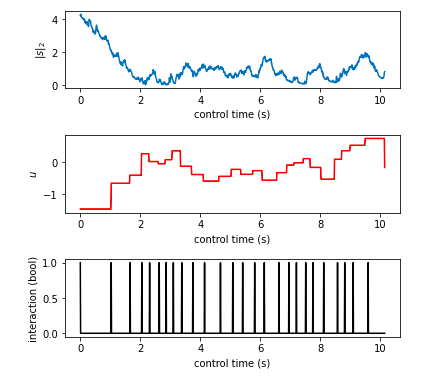
\includegraphics[width=8cm]{naiive.png}
 	\caption{A control path with learned policy $\hat{\pi}_{\textrm{MB}}$} \label{naiive}
\end{figure}
In Figure \ref{naiive}, the norm of state $s$, the control signal $u$ and the boolean which denotes whether agent interact with environment at time $t$ second are shown from top to bottom.


\subsubsection{Result of Proposed Method}
First, we consider the results of reinforcement learning using the proposed method 1 with $\hat{\pi}^{\textrm{MB}}$ as the initial policy. Figure \ref{proposed_1_linear} shows the path controlled by the policy $\pi_{\textrm{prop}}^L$ from the initial state $s_0=\begin{bmatrix}3 & 3\end{bmatrix}$.
\begin{figure}[H]
	\centering
 	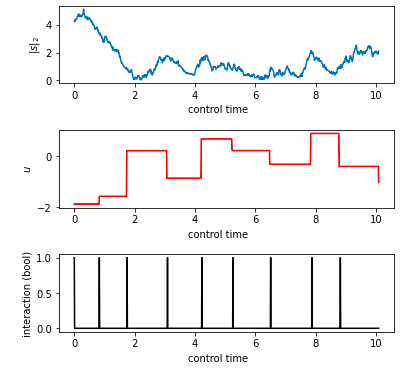
\includegraphics[width=8cm]{proposed_1_linear.png}
 	\caption{A control path with learned policy $\pi_{\textrm{prop}}^L$} \label{proposed_1_linear}
\end{figure}
The evaluation value of this policy $\pi_{\textrm{prop}}^L$ is
\begin{equation}
	\tilde{J}(\pi_{\textrm{prop}}^L) \simeq -11.986561081591695.
\end{equation}
Thus, we can see the improvement of policy from $\pi_{\textrm{MB}}$.\par
The change of the value of the evaluation function $J( \pi_{\theta})$ as the policy parameter $\theta$ is updated is shown in Figure \ref{evaluation_log_linear}.
\begin{figure}[H]
	\centering
 	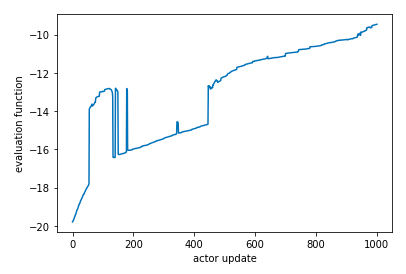
\includegraphics[width=10cm]{evaluation_log_linear.png}
 	\caption{Policy improvement on linear case} \label{evaluation_log_linear}
\end{figure}
Figure \ref{evaluation_log_linear} shows an example of successful learning. However, since the calculation of the policy gradient depends on the approximation accuracy of the critic according to the equation \eqref{app_pg_stc}, we often observed a sharp deterioration of the policy using the proposed method. Therefore, the learning accuracy of critic is a future work.

\if0
\subsubsection{Proposed Method 2}
As mentioned in section \ref{sec:other_approach}, in the proposed method 2, there are two possibilities to minimize the value function \eqref{other} for state $s$ as follows:
\begin{itemize}
	\item To enlarge the communication interval while keeping the control cost low.
	\item To communicate in small increments, and to reduce the accumulated cost by the discount rate.
\end{itemize}
In fact, after several episodes of reinforcement learning with 1000000 steps using the proposed method 2, we obtained control policies shown in Figure \ref{proposed_2_large} and Figure \ref{proposed_2_small}. 
\begin{figure}[h]%%%%%%
	\centering
 	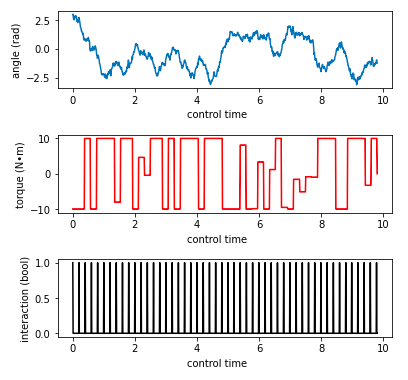
\includegraphics[width=8cm]{sample_02.png}
 	\caption{A control path with initial policy $\pi_{\textrm{prop}2}^L$} \label{proposed_2_large}
\end{figure}\\
\begin{figure}[h]
	\centering
 	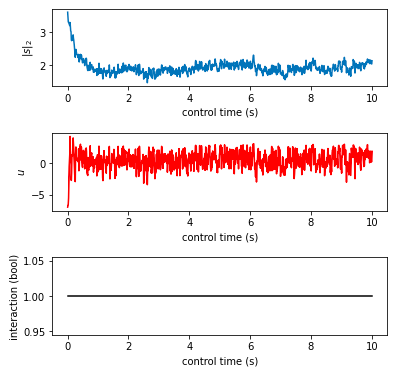
\includegraphics[width=8cm]{proposed_2_small.png}
 	\caption{A control path with initial policy $\pi_{\textrm{prop}2}^S$} \label{proposed_2_small}
\end{figure}\\

Let denote these policies as $\pi_{\textrm{prop}2}^L$ and $\pi_{\textrm{prop}2}^S$, respectively, and the value of the evaluation function \eqref{evaluation} is 
\begin{align}
	J(\pi_{\textrm{prop}2}^L) &= \\
	J(\pi_{\textrm{prop}2}^S) &= -479.71211911203886.
\end{align}
Therefore, there is a possibility that the proposed method 2 can be used to learn policies that reduce the evaluation function \eqref{evaluation}, but we cannot guarantee it. 
\fi

\subsection{Non-Linear Case}
In this subsection, we investigate whether the self-triggered control law can be learned by reinforcement learning even when the control target is extended to non-linear systems, especially control affine systems. We consider an inverted pendulum, whose state-space representation is
\begin{equation}
	\odif{}{t}\begin{bmatrix}\theta \\ \dot{\theta}\end{bmatrix} = 
		\begin{bmatrix}\dot{\theta} \\ \frac{3g}{2l}\sin{\theta} + \frac{3}{ml^2}a \end{bmatrix} + \begin{bmatrix}1 \\ 1\end{bmatrix}\dot{w}\label{pendulum}.
\end{equation}
where $\dot{w}$ is wiener process noise. Therefore, for an inverted pendulum, the state variable $s$ is considered to be $\begin{pmatrix}\theta & \dot{\theta}\end{pmatrix}^{\top}$.
\par
As in the linear case, the input signal $u$ is limited to $-10 \sim 10$. And let the state spase be $S = \{s\in \mathbb{R}^2| s_0\in[-\pi,\pi], s_1\in[-2\pi,2\pi]\}$. If angle $\|\theta\| > \pi$, $\theta$ will be  replaced by the equivalent angle which satisfies $\|\theta\| \leq \pi$. And if Angular velocity $\|\dot{\theta}\| > 2\pi$, $\|\dot{\theta}\|$ will be clipped.

\subsubsection{Initial Policy}
The initial policy $\pi_{\textrm{init}}$ used in this case is
\begin{equation}
	\pi_{\textrm{init}}(s) = \begin{bmatrix}-Ks&0.2\end{bmatrix}
\end{equation}
where $K$ is a feedback gain calculated by Linear Quadratic Regulator for linearized system around $s = \bm{0}$. Figure \ref{sample_02} shows the control path with initial policy $\pi_{\textrm{init}}$ stating from $s_0 = [3., 3.]$.
\begin{figure}[h]
	\centering
 	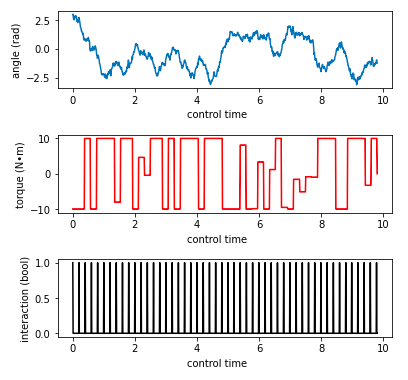
\includegraphics[width=8cm]{sample_02.png}
 	\caption{A control path with initial policy $\pi_{\textrm{init}}$} \label{sample_02}
\end{figure}\\
The evaluation value of $\pi_{\textrm{init}}$ is
\begin{equation}
	\tilde{J}(\pi_{\textrm{init}}) \simeq -62.492721990335504.
\end{equation}
In Figure \ref{sample_02}, the angle of pendulum $\theta$ rad, the torque $u$ N$\cdot$m and the boolean which denotes whether agent interact with environment at time $t$ second are shown from top to bottom.


\subsubsection{Result of Proposed Method}
First, we show the results of reinforcement learning by the proposed method 1. Figure \ref{proposed_1_nl} shows the control path by the obtained policy $\pi_{\textrm{prop}}^N$ stating from $s_0 = [3., 3.]$.
\begin{figure}[H]
	\centering
 	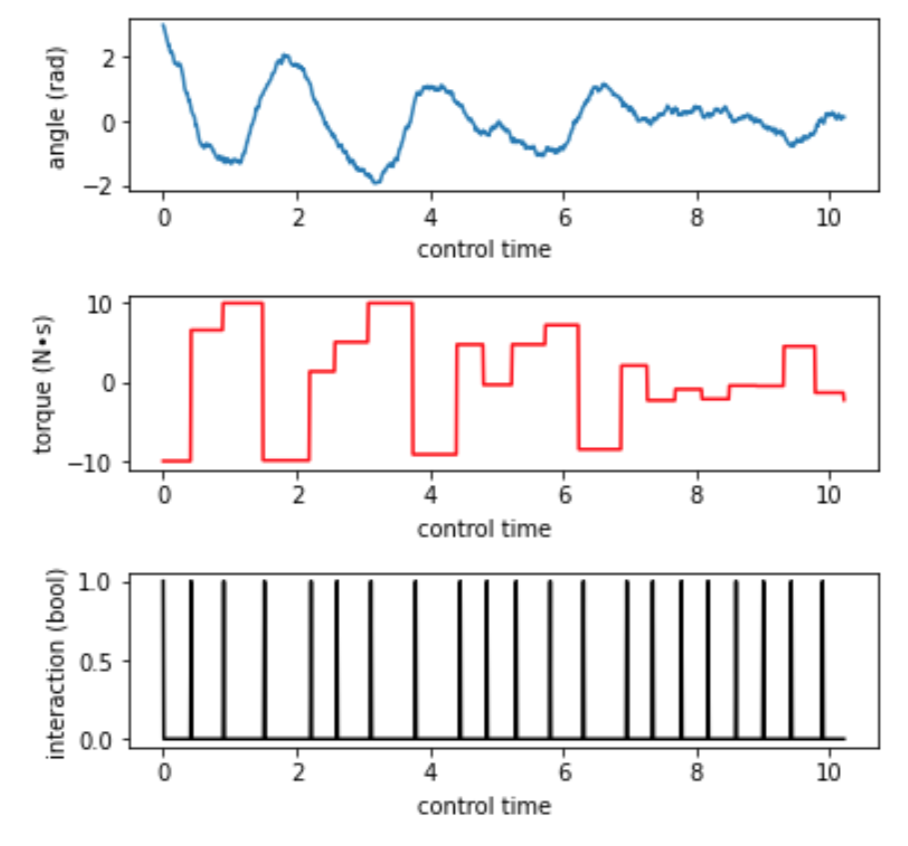
\includegraphics[width=8cm]{proposed_1_nl.png}
 	\caption{A control path with learned policy $\pi_{\textrm{prop}}^N$} \label{proposed_1_nl}
\end{figure}
The evaluation value of $\pi_{\textrm{prop}}^N$ is
\begin{equation}
	\tilde{J}(\pi_{\textrm{prop}}^N) \simeq -33.49714598533895.
\end{equation}\\
Thus, we can confirm the improvement of policy.\par
The change of the value of the evaluation function $J( \pi_{\theta})$ as the policy parameter $\theta$ is updated is shown in Figure \ref{evaluation_log_nl}.
\begin{figure}[H]
	\centering
 	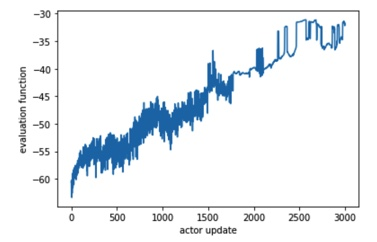
\includegraphics[width=10cm]{evaluation_log_nl.png}
 	\caption{Policy improvement on non-linear case} \label{evaluation_log_nl}
\end{figure}

\if0
\subsubsection{Proposed Method 2}
As in the linear case, reinforcement learning with the proposed method 2 for 1000000 steps yields two kinds of policies: one is to reduce the control cost while increasing the communication interval, and the other is to minimize the evaluation function by making the communication detailed. Figures \ref{nonlinear_good} and \ref{nonlinear_bad} show the control paths of $\pi_{\textrm{prop}2}^L$ and $\pi_{\textrm{prop}2}^S$, respectively.
\begin{figure}[h]
	\centering
 	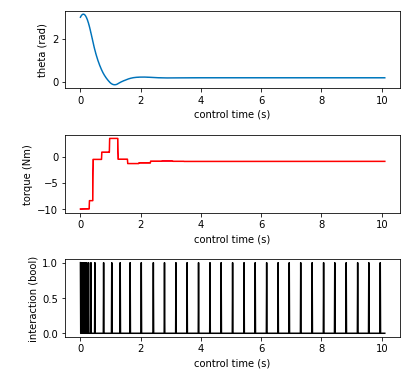
\includegraphics[width=8cm]{path_1.png}
 	\caption{A control path with learned policy $\pi_{\textrm{RL}}$} \label{nonlinear_good}
\end{figure}\\
\begin{figure}[h]
	\centering
 	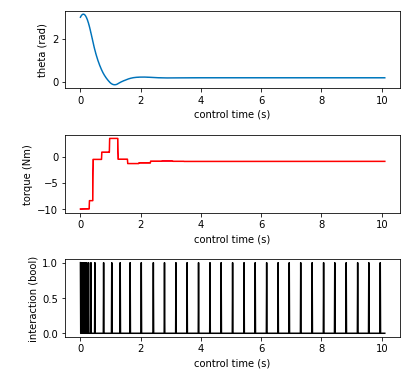
\includegraphics[width=8cm]{path_1.png}
 	\caption{A control path with learned policy $\pi_{\textrm{RL}}$} \label{nonlinear_bad}
\end{figure}
The values of the evaluation functions \ref{evaluation} are 
\begin{align}
	J(\pi_{\textrm{prop}2}^L) &= \\
	J(\pi_{\textrm{prop}2}^S) &= .
\end{align}
Therefore, as in the linear case, it is possible that the proposed method 2 can be used to learn a policy that reduces the evaluation function, but we cannot guarantee it. 
\fi

\section{Conclusion}
In this paper, we formulate an optimal self-triggered control problem where communication cost is explicitly included, which has not been considered in previous studies. Then, we consider a reinforcement learning approach to the problem.  \par
First, from the configuration of the evaluation function, we confirm that the deterministic policy gradient theorem for general reinforcement learning is not directly applicable, and then we derive a policy gradient theorem that is compatible with the formulated optimal self-triggered control problem. \par
In this paper, we also propose a reinforcement learning algorithm for approximate computation of the policy gradient. As a result of the implementation, for the linear system, we can improve the policy in the sense of the formulated evaluation function for the control law designed naively in the model base. We also succeeded in improving the policy for self-triggered control of nonlinear systems, which was not solved in the previous study. \par
However, the computational complexity and the way of saving the empirical data are important issues to be solved in the future, because they greatly affect the results of the calculation of the policy gradient.

%%% Acknowledgments %%%%%%%%%%%%%%%%%%%%%%%%%%%%%%%%%%%%%%%%%%%%%%%%%%%%%%%%%%%%%
\acknowledgment
The author would like to express his sincere gratitude to Professor
Yoshito Ohta and Assistant Professor Kenji Kashima for their helpful advices.

%%% References %%%%%%%%%%%%%%%%%%%%%%%%%%%%%%%%%%%%%%%%%%%%%%%%%%%%%%%%%%%%%%%%%%
\addcontentsline{toc}{section}{\refname} % Add to the table of contents.
                                         % Delete if you use chapter option.
\begin{thebibliography}{20}
\bibitem{ETC_intro}
W. P. M. H. Heemels, K. H. Johansson, and P. Tabuada. “An intro- duction to event-triggered and self-triggered control.” \textit{In Proc. of the 51st IEEE International Conference on Decision and Control}, 2012.
\bibitem{ETC}
D. Baumann, J. J. Zhu, G. Martius, and S. Trimpe. “Deep Reinforcement Learning for Event-Triggered Control.”  \textit{In Proc. of the 57th IEEE International Conference on Decision and Control}, 2018.
\bibitem{STC}
T. Gommans, D. Antunes, T. Donkers, P. Tabuada, and M. Heemels. “Self-triggered linear quadratic control.” \textit{Automatica}, vol. 50, no. 4, pp. 1279-1287, 2014.
\bibitem{ECBF}
G. Yang, C. Belta, and R. Tron. “Self-triggered Control for Safety Critical Systems Using Control Barrier Functions."  \textit{In American Control Conference (ACC) Philadelphia, USA}, 2019.
\bibitem{Q}
C. J. Watkins, and P. Dayan. Q-learning. \textit{Machine Learning}, vol. 8, no. 3-4, pp. 279-292, 1992.
\bibitem{DQN}
V. Minh, K. Kavukcouglu, D. Silver. et al.. “Human-level control through deep reinforcement learning." \textit{Nature 518}, pp.529-533, 2015.
\bibitem{DPG}
D. Silver, G. Lever, N. Heess, T. Degris, D. Wierstra, et al.. “Deterministic Policy Gradient Algorithms." \textit{ICML Beijing, China.}, 2014, Beijing.
\bibitem{DDPG}
T. P. Lillicrap, J. J. Hunt, A. Pritzel, N.Heess, T. Erez, Y. Tassa, D. Silver, and D. Wierstra. Continuous control with deep reinforcement learning. \textit{International Conference on Learning Representations}, 2015.
\bibitem{survey}
I. Grondman, L. Busoniu, G. A. Lopes, and R. Babuska. “A Survey of Actor-Critic Reinforcement Learning: Standard and Natural Policy Gradient." \textit{IEEE Transactions on Systems, Man, and Cybernetics, Part C (Applications and Reviews)}, 42(6):1291-1307, 2012.
\bibitem{off-PAC}
T. Degris, M. White and R. Sutton. “Off-Policy Actor-Critic." \textit{ICML Edinburgh, United Kingdom}, 2012.
\bibitem{approximation}
R. S. Sutton, D. McAllester, S. Singh, and Y. Mansour. "Policy gradient methods for reinforcement learning with function approximation." \textit{In Advances in Neural Information Processing Systems}, 2000.
\bibitem{Adam}
D. P. Kingma and J. Ba. “Adam: A Method for Stochastic Optimization." \textit{arXiv preprint arXiv: 1412.6980}, 2014.

\end{thebibliography}
%%% If you want to use BibTeX, delete the above and insert code here.
%% \bibliographystyle{...}
%% \bibliography{...}

%%% Appendix %%%%%%%%%%%%%%%%%%%%%%%%%%%%%%%%%%%%%%%%%%%%%%%%%%%%%%%%%%%%%%%%%%%%
%%% If you don't need appendices, delete the below.
\appendix

\section{Appendix}
\subsection{Model Settings}
We use DDPG as reinforcement learning algorithm. As described in section 2, actor and critic is expressed as neural networks respectively. Experiments have shown that learning diverges when using a general network, so here we use the special network. The architecture of 2 networks is in Fig \ref{NN}.
\begin{figure}[h]
	\centering
 	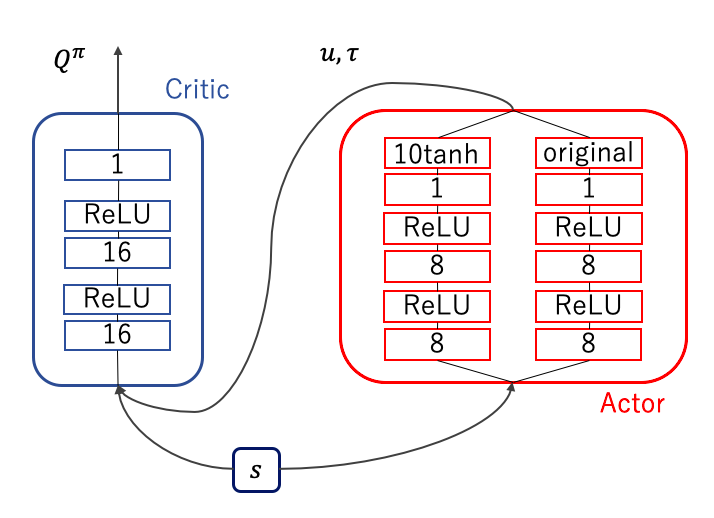
\includegraphics[width=10cm]{model.png}
 	\caption{Agent Model} \label{NN}
\end{figure}\\
The activation function "original" shown in Fig \ref{NN} is defined as $0.99 \times \textrm{sigmoid} + 0.01$ to meet upper and lower limits of interval described in the next section.\par

%%% End of body %%%%%%%%%%%%%%%%%%%%%%%%%%%%%%%%%%%%%%%%%%%%%%%%%%%%%%%%%%%%%%%%%
\fi
\ifoutputcover
\cleardoublepage
%%% Covers and abstract for submission %%%%%%%%%%%%%%%%%%%%%%%%%%%%%%%%%%%%%%%%%%
\makecover                      % Cover
\makespine[\numberofspines]     % Spine
\fi
\ifoutputabstractforsubmission
\makeabstractforsubmission      % Abstract for submission
\fi
\end{document}
